\section{Management der Software-Entwicklung}

\paragraph{Themen dieses Kapitels}
\begin{itemize}
	\item bessere/modernere Prozessmodelle
	\item Verbesserung/Qualität von Softwareprozessmodellen
	\item Projektmanagement(-werkzeuge)
	\item optional: Kostenschätzung für Softwareprojekte
\end{itemize}

Viele im folgenden vorgestellten Überlegungen sind nicht ausschließlich für \textbf{Software} Entwicklungsprozesse geeignet, sondern werden ganz allgemein für die Steuerung komplexer technischer Entwicklungsprozesse eingesetzt.

\paragraph{Aufgaben des Managements:}
\begin{itemize}
	\item \textbf{Planungsaktivitäten}: Ziele definieren, Vorgehensweisen auswählen, Termine fest legen, Budgets vorbereiten, ...
	\begin{itemize}
		\item Vorgehensmodelle, Kostenschätzung, Projektpläne
	\end{itemize}
	\item \textbf{Organisationsaktivitäten}: Strukturieren von Aufgaben, Festlegung organisatorischer Strukturen, Definition von Qualifikationsprofilen für Positionen, ...
	\begin{itemize}
		\item Rollenmodelle, Team-Modelle, Projektpläne
	\end{itemize}
	\item \textbf{Personalaktivitäten}: Positionen besetzen, Mitarbeiter beurteilen, weiterbilden, ...
	\begin{itemize}
		\item nicht Thema dieser Vorlesung
	\end{itemize}
	\item  \textbf{Leitungsaktivitäten}: Mitarbeiter führen, motivieren, koordinieren, ...
	\begin{itemize}
		\item nicht Thema dieser Vorlesung
	\end{itemize}
	\item  \textbf{Kontrollaktivitäten}: Prozess- und Produktstandards entwickeln, Berichts- und Kontrollwesen etablieren, Prozesse und Produkte vermessen, Korrekturen, ...
	\begin{itemize}
		\item Qualititätsmanagement, insbesondere für Software-Entwicklungsprozesse
	\end{itemize}
\end{itemize}

\paragraph{Ziele des Managements}

Hauptziel des Projektmanagements ist die \textbf{Erhöhung der Produktivität}! 
\\ 
\\
\textbf{Allgemeine Definition von Produktivität:} Produktivität = Produktwert / Aufwand (oder: Leistung / Aufwand)
\\
\\
\textbf{Für Software-Entwicklung oft verwendete Definition:} Produktivität = Größe der Software / geleistete Mitarbeitertage
\begin{itemize}
	\item Maß für Größe der Software
	\item Berücksichtigung der Produktqualität
	\item Aufwand = Mitarbeitertage ?
	\item Nutzen (Return Of Investment) = Größe der Software ?
\end{itemize}

\paragraph{Einflussfaktoren für Produktivität [ACF97]:}
Angabe der Form ''+ 1 : X'' steht für Produktivitätssteigerung um maximal Faktor X \\
Angabe der Form ''- 1 : Y'' steht für Produktivitätsminderung um maximal Faktor Y.
\begin{itemize}
	\item Werkzeug-Einsatz: + 1 : 1,6
	\item Geeignete Methoden: + 1 : 1,9
	\item Produktkomplexität: - 1 : 2,4
	\item Hohe Zuverlässigkeitsanforderung: - 1 : 1,9
	\item Firmenkultur (corporate identity): + 1 : 11
	\item Arbeitsumgebung (eigenes Büro, abschaltbares Telefon, ... ): + 1 : ???
	\item Begabung der Mitarbeiter: + 1 : 10
	\item Erfahrung im Anwendungsgebiet: + 1 : 1,6
	\item Bezahlung, Berufserfahrung: kein messbarer Einfluss
\end{itemize}

\subsection{''Neuere'' Vorgehensmodelle}
Die naheliegendste Idee zur Verbesserung des Wasserfallmodells ergibt sich durch die Einführung von \textbf{Zyklen} bzw. \textbf{Rückgriffen}. Sie erlauben Wiederaufnehmen früherer Phasen, wenn in späteren Phasen Probleme auftreten.
\paragraph{Weitere Vorgehensmodelle:}
\begin{itemize}
	\item das V-Modell (umgeklapptes Wasserfallmodell)
	\item das evolutionäre Modell (iteriertes Wasserfallmodell)
	\item Rapid Prototyping (Throw-Away-Prototyping)
\end{itemize}

\paragraph{Probleme mit dem Wasserfallmodell insgesamt:}
\begin{itemize}
	\item Wartung mit ca. 60\% des Gesamtaufwandes ist eine Phase
	\begin{itemize}
		\item andere Prozessmodelle mit Wartung als eigener Entwicklungsprozess
	\end{itemize}
	\item zu Projektbeginn sind nur ungenaue Kosten- und Ressourcenschätzungen möglich
	\begin{itemize}
		\item Methoden zur Kostenschätzung anhand von Lastenheft (Pflichtenheft)
	\end{itemize}
	\item ein Pflichtenheft kann nie den Umgang mit dem fertigen System ersetzen, das erst sehr spät entsteht (Risikomaximierung)
	\begin{itemize}
		\item andere Prozessmodelle mit Erstellung von Prototypen, ...
	\end{itemize}
	\item Anforderungen werden früh eingefroren, notwendiger Wandel (aufgrund organisatorischer, politischer, technischer, ... Änderungen) nicht eingeplant
	\begin{itemize}
		\item andere Prozessmodelle mit evolutionärer Software-Entwicklung
	\end{itemize}
	\item strikte Phaseneinteilung ist unrealistisch (Rückgriffe sind notwendig)
	\begin{itemize}
		\item andere Prozessmodelle mit iterativer Vorgehensweise
	\end{itemize}
\end{itemize}

\begin{figure}[h]
	\centering
	\caption{Evolutionäres Modell (evolutionäres Prototyping)}
	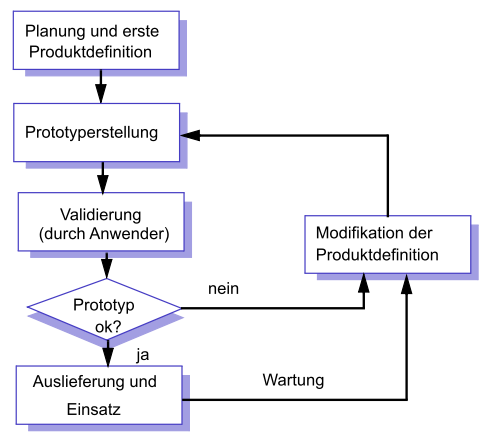
\includegraphics[width=0.5\textwidth]{5_1_1}
\end{figure}

\paragraph{Bewertung des evolutionären Modells:}
\begin{itemize}
	\item \textbf{Vorteile:}
	\begin{itemize}
		\item es ist sehr früh ein (durch Kunden) evaluierbarer Prototyp da
		\item Kosten und Leistungsumfang des gesamten Softwaresystems müssen nicht zu Beginn des Projekts vollständig festgelegt werden
		\item Projektplanung vereinfacht sich durch überschaubarere Teilprojekte
		\item  Systemarchitektur muss auf Erweiterbarkeit angelegt sein
	\end{itemize}
	\item \textbf{Nachteile:}
	\begin{itemize}
		\item es ist schwer, Systemarchitektur des ersten Prototypen so zu gestalten, dass sie alle später notwendigen Erweiterungen erlaubt
		\item Prozess der Prototyperstellung nicht festgelegt: Spiralmodell von Berry Böhm integriert Phasen des Wasserfallmodells
		\item evolutionäre Entwicklung der Anforderungsdefinition birgt Gefahr in sich, dass bereits realisierte Funktionen hinfällig werden
		\item  Endresultat sieht ggf. wie Software nach 10 Jahren Wartung aus
	\end{itemize}
\end{itemize}

\paragraph{Rapid Prototyping (Throw-Away-Prototyping):}
Mit Generatoren, ausführbaren Spezifikationssprachen, Skriptsprachen etc. wird:
\begin{itemize}
	\item Prototyp des Systems (seiner Benutzeroberfläche) realisiert
	\item dem Kunden demonstriert
	\item und anschließend weggeschmissen
\end{itemize}
\textbf{Bewertung:}
\begin{itemize}
	\item erlaubt schnelle Klärung der Funktionalität und Risikominimierung
	\item Vermeidung von Missverständnissen zwischen Entwickler und Auftraggeber
	\item früher Test der Benutzerschnittstelle
\end{itemize}

\subsection{Rational Unified Process für UML}
\begin{figure}[h]
	\centering
	\caption{Firma IBM (ehemals Rational) dominiert(e) Entwicklung der Standard-OO-Modellierungssprache UML und des zugehörigen Vorgehensmodells.}
	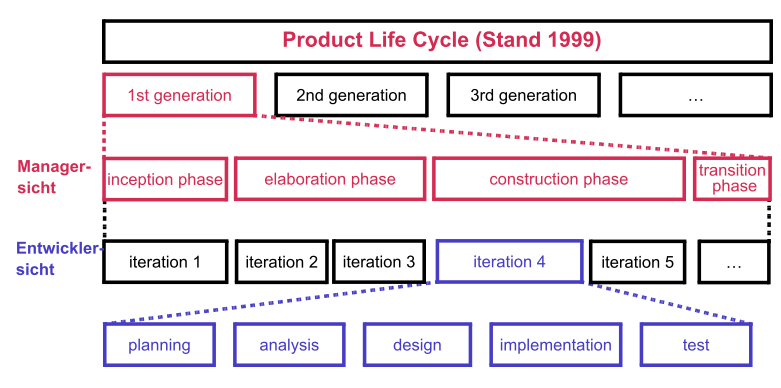
\includegraphics[width=0.85\textwidth]{5_2}
\end{figure}

\paragraph{Phasen der Lebenszyklusgeneration}
\begin{itemize}
	\item \textbf{Inception (Vorbereitung)}: Definition des Problembereichs und Projektziels für Produktgeneration mit Anwendungsbereichsanalyse (Domain Analysis) und Machbarkeitsstudie (für erste Generation aufwändiger)
	\begin{itemize}
		\item bei Erfolg weiter zu ...
	\end{itemize}
	\item \textbf{Elaboration (Entwurf)}: erste Anforderungsdefinition für Produktgeneration mit grober Softwarearchitektur und Projektplan (ggf. mit Rapid Prototyping)
	\begin{itemize}
		\item bei Erfolg weiter zu ...
	\end{itemize}
	\item  \textbf{Construction (Konstruktion)}: Entwicklung der neuen Produktgeneration als eine Abfolge von Iterationen mit Detailanalyse, -design, ... (wie beim evolutionären Vorgehensmodell)
	\begin{itemize}
		\item bei Erfolg weiter zu ...
	\end{itemize}
	\item  \textbf{Transition (Einführung)}: Auslieferung des Systems an den Anwender (inklusive Marketing, Support, Dokumentation, Schulung, ... )
\end{itemize}

\paragraph{Eigenschaften des Rational Unified Prozesses (RUP):}
\begin{itemize}
	\item  \textbf{modellbasiert}: für die einzelnen Schritte des Prozesses ist festgelegt, welche Modelle (Dokumente) des Produkts zu erzeugen sind
	\item \textbf{prozessorientiert}: die Arbeit ist in eine genau definierte Abfolge von Aktivitäten unterteilt, die von anderen Teams in anderen Projekten wiederholt werden können.
	\item \textbf{iterativ und inkrementell}: die Arbeit ist in eine Vielzahl von Iterationen unterteilt, das Produkt wird inkrementell entwickelt.
	\item \textbf{risikobewusst}: Aktivitäten mit hohem Risiko werden identifiziert und in frühen Iterationen in Angriff genommen.
	\item \textbf{zyklisch}: die Produktentwicklung erfolgt in Zyklen (Generationen). Jeder Zyklus liefert eine neue als kommerzielles Produkt ausgelieferte Systemgeneration.
	\item \textbf{ergebnisorientiert}: jede Phase (Iteration) ist mit der Ablieferung eines definierten Ergebnisses meist zu einem konkreten Zeitpunkt (Meilenstein) verbunden
\end{itemize}

\paragraph{Faustregeln für die Ausgestaltung eines Entwicklungsprozesses:}
\begin{itemize}
	\item die Entwicklung einer \textbf{Produktgeneration} dauert höchstens 18 Monate
	\item eine \textbf{Vorbereitungsphase} dauert 3-6 Wochen und besteht aus einer Iteration
	\item eine \textbf{Entwurfsphase} dauert 1-3 Monate und besteht aus bis zu 2 Iterationen
	\item  eine \textbf{Konstruktionsphase} dauert 1-9 Monate und besteht aus bis zu 7 Iterationen
	\item eine \textbf{Einführungsphase} dauert 4-8 Wochen und besteht aus einer Iteration
	\item jede \textbf{Iteration} dauert 4-8 Wochen (ggf. exklusive Vorbereitungs- und Nachbereitungszeiten, die mit anderen Iterationen überlappen dürfen)
	\item das gewünschte \textbf{Ergebnis} (Software-Release) einer Iteration ist spätestens bei ihrem Beginn festgelegt (oft Abhängigkeit von Ergebnissen vorheriger Iterationen)
	\item die \textbf{geplante Zeit} für eine Iteration wird nie (höchstens um 50\%) überschritten
	\item innerhalb der Konstruktionsphase wird mindestens im wöchentlichen Abstand ein \textbf{internes Software-Release} erstellt
	\item  mindestens 40\% \textbf{Reserve} an Projektlaufzeit für unbekannte Anforderungen, ...
\end{itemize}

\paragraph{Anmerkungen zu den Arbeitsbereichen (Workflows) des RUP:}
\begin{itemize}
	\item \textbf{Business Modeling} befasst sich damit, das Umfeld des zu erstellenden Softwaresystems zu erfassen (Geschäftsvorfälle, Abläufe, ... )
	\item \textbf{Requirements (Capture)} befasst sich damit die Anforderungen an ein Softwaresystem noch sehr informell zu erfassen
	\item \textbf{Analysis/Design} präzisiert mit grafischen Sprachen (Klassendiagramme etc.) die Anforderungen und liefert Systemarchitektur
	\item \textbf{Implementation/Test} entspricht den Aktivitäten in den Phasen ''Codierung bis Integrationstest'' des Wasserfallmodells
	\item \textbf{Deployment} entspricht ''Auslieferung und Installation'' des Wasserfallmodells
	\item \textbf{Configuration Management} befasst sich mit der Verwaltung von Softwareversionen und -varianten
	\item \textbf{Project Management} mit der Steuerung des Entwicklungsprozesses selbst
	\item \textbf{Environment} bezeichnet die Aktivitäten zur Bereitstellung benötigter Ressourcen (Rechner, Werkzeuge, ... )
\end{itemize}

\paragraph{Bewertung des (Rational) Unified Prozesses:}
\begin{itemize}
	\item Vorteile
	\begin{itemize}
		\item Manager hat die grobe ''Inception-Elaboration-Construction-Transition''-Sicht
		\item Entwickler hat zusätzlich die feinere arbeitsbereichsorientierte Sicht
		\item Wartung ist eine Abfolge zu entwickelnder Produktgenerationen
		\item es wird endgültig die Illusion aufgegeben, dass Analyse, Design, ... zeitlich begrenzte strikt aufeinander folgende Phasen sind
		\item es gibt ''Open Unified Process'' im Eclipse Umfeld
	\end{itemize}
	\item Nachteile
	\begin{itemize}
		\item sehr komplexes Vorgehensmodell für modellbasierte SW-Entwicklung
		\item nicht mit Behördenstandards (V-Modell, ... ) richtig integriert
		\item Qualitätssicherung ist kein eigener Aktivitätsbereich
	\end{itemize}
\end{itemize}

\subsection{Leichtgewichtige Prozessmodelle}

Herkömmlichen Standards für Vorgehensmodelle zur Softwareentwicklung (V-Modell, RUP) wird vorgeworfen, dass
\begin{itemize}
	\item sie sehr starr sind
	\item Unmengen an Papier produzieren
	\item und nutzlos Arbeitskräfte binden
\end{itemize}
Deshalb werden seit einiger Zeit sogenannte ''leichtgewichtige'' Prozessmodelle (\textbf{light-weight processes}) unter dem Schlagwort ''Agile Prozessmodelle'' propagiert, die sinnlosen bürokratischen Overhead vermeiden wollen.
\begin{itemize}
	\item siehe separater Foliensatz zu dieser Thematik
\end{itemize}

\paragraph{Verbesserung der Prozessqualität}
Ausgangspunkt der hier vorgestellten Ansätze sind folgende Überlegungen:
\begin{itemize}
	\item Softwareentwicklungsprozesse sind selbst Produkte, deren Qualität überwacht und verbessert werden muss
	\item bei der Softwareentwicklung sind bestimmte Standards einzuhalten (Entwicklungsprozess muss dokumentiert und nachvollziehbar sein)
	\item es bedarf kontinuierlicher Anstregungen, um die Schwächen von Entwicklungsprozessen zu identifizieren und zu eliminieren
\end{itemize}


\textbf{Hier vorgestellte Ansätze:}
\begin{itemize}
	\item \textbf{ISO 9000 Normenwerk} (Int. Standard für die Softwareindustrie)
	\item \textbf{Capability Maturity Model} (CMM/CMMI) des Software Engineering 
	Institutes (SEI) an der Carnegie Mellon University
	\item ISO-Norm \textbf{SPiCE} integriert und vereinheitlicht CMM und ISO 9000
\end{itemize}

\paragraph{Qualitätssicherung mimt der ISO 9000:}
Das \textbf{ISO 9000 Normenwerk} legt für das Auftraggeber-Lieferantenverhältnis einen allgemeinen organisatorischen Rahmen zur Qualitätssicherung fest.
\\
\\
Das ISO 9000 Zertifikat bestätigt, dass die Verfahren eines Unternehmens der ISO 9000 Norm entsprechen.

\paragraph{Wichtige Teile:}
\begin{itemize}
	\item \textbf{ISO 9000-1}: allgemeine Einführung und Überblick
	\item \textbf{ISO 9000-3}: Anwendung von ISO 9001 auf Softwareproduktion
	\item \textbf{ISO 9001}: Modelle der Qualitätssicherung in Design/Entwicklung, Produktion, Montage und Kundendienst
	\item \textbf{ISO 9004}: Aufbau und Verbesserung eines Qualitätsmanagementsystems
\end{itemize}

\paragraph{Von ISO 9000-3 vorgeschriebene Dokumente:}
\begin{itemize}
	\item \textbf{Vertrag Auftraggeber - Lieferant:}  Tätigkeiten des Auftraggebers, Behandlung von Anforderungsänderungen, Annahmekriterien (Abnahmetest), ...
	\item \textbf{Spezifikation:} funktionale Anforderungen, Ausfallsicherheit, Schnittstellen, ... des Softwareprodukts
	\item \textbf{Entwicklungsplan:} Zielfestlegung, Projektmittel, Entwicklungsphasen, Management, eingesetzte Methoden und Werkzeuge, ...
	\item \textbf{Qualitätssicherungsplan:}  Qualitätsziele (messbare Größen), Kriterien für Ergebnisse v. Entwicklungsphasen, Planung von Tests, Verifikation, Inspektionen
	\item \textbf{Testplan:} Teststrategie (für Integrationstest), Testfälle, Testwerkzeuge, Kriterien für Testvollständigkeit/Testende
	\item \textbf{Wartungsplan:} Umfang, Art der Unterstützung, ...
	\item \textbf{Konfigurationsmanagement:} Plan für Verwaltung von Softwareversionen und Softwarevarianten
\end{itemize}

\paragraph{Von ISO 9000-3 vorgeschriebene Tätigkeiten:}
\begin{itemize}
	\item \textbf{Konfigurationsmanagement} für Identifikation und Rückverfolgung von Änderungen, Verwaltung parallel existierender Varianten
	\item \textbf{Dokumentenmanagement} für geordnete Ablage und Verwaltung aller bei der Softwareentwicklung erzeugten Dokumente
	\item \textbf{Qualitätsaufzeichungen} (Fehleranzahl oder Metriken) für Verbesserungen am Produkt und Prozess
	\item \textbf{Festlegung} von Regeln, Praktiken und Übereinkommen für ein Qualitätssicherungssystem
	\item \textbf{Schulung} aller Mitarbeiter sowie Verfahren zur Ermittlung des Schulungsbedarfes
\end{itemize}
\textbf{Zertifizierung:} Die Einhaltung der Richtlinien der Norm wird von unabhängigen Zertifizierungsstellen im jährlichen Rhythmus überprüft.

\paragraph{Bewertung von ISO 9000:}
\begin{itemize}
	\item Vorteile
	\begin{itemize}
		\item lenkt die Aufmerksamkeit des Managements auf Qualitätssicherung
		\item ist ein gutes Marketing-Instrument
		\item reduziert das Produkthaftungsrisiko (Nachvollziehbarkeit von Entscheidungen)
	\end{itemize}
	\item Nachteile
	\begin{itemize}
		\item Nachvollziehbarkeit und Dokumentation von Prozessen reicht aus
		\item keine Aussage über Qualität von Prozessen und Produkten
		\item (für kleine Firmen) nicht bezahlbarer bürokratischer Aufwand
		\item Qualifikation der Zertifizierungsstellen umstritten
		\item oft große Abweichungen zwischen zertifiziertem Prozess und realem Prozess
	\end{itemize}
\end{itemize}

\paragraph{Das Capability Maturity Model (CMM):}
Referenzmodell zur Beurteilung von Softwarelieferanten, vom Software Engineering Institute entwickelt
\begin{itemize}
	\item Softwareentwicklungsprozesse werden in \textbf{5 Reifegrade} unterteilt
	\item Reifegrad (\textbf{maturity}) entspricht Qualitätsstufe der Softwareentwicklung
	\item höhere Stufe beinhaltet Anforderungen der tieferen Stufen
\end{itemize}

\textbf{Stufe 1 - chaotischer initialer Prozess (ihr Stand vor dieser Vorlesung):}
\begin{itemize}
	\item Prozess-Charakteristika:
	\begin{itemize}
		\item unvorhersehbare Entwicklungskosten, -zeit und -qualität
		\item kein Projektmanagement, nur ''Künstler'' am Werke
	\end{itemize}
	\item notwendige Aktionen:
	\begin{itemize}
		\item Planung mit Kosten- und Zeitschätzung einführen
		\item Änderungs- und Qualitätssicherungsmanagement 
	\end{itemize}
\end{itemize}

\textbf{Stufe 2 - wiederholbarer intuitiver Prozess  (Stand nach dieser Vorlesung?):}
\begin{itemize}
	\item Prozess-Charakteristika:
	\begin{itemize}
		\item Kosten und Qualität schwanken, gute Terminkontrolle
		\item Know-How einzelner Personen entscheidend
	\end{itemize}
	\item notwendige Aktionen:
	\begin{itemize}
		\item Prozessstandards entwickeln
		\item Methoden (für Analyse, Entwurf, Testen, ... ) einführen
	\end{itemize}
\end{itemize}

\textbf{Stufe 3 - definierter qualitativer Prozess (Stand der US-Industrie 1989?):}
\begin{itemize}
	\item Prozess-Charakteristika:
	\begin{itemize}
		\item zuverlässige Kosten- und Terminkontrolle, schwankende Qualität
		\item institutionalisierter Prozess, unabhängig von Individuen
	\end{itemize}
	\item notwendige Aktionen:
	\begin{itemize}
		\item Prozesse vermessen und analysieren
		\item quantitative Qualitätssicherung
	\end{itemize}
\end{itemize}

\textbf{Stufe 4 - gesteuerter/geleiteter quantitativer Prozess:}
\begin{itemize}
	\item Prozess-Charakteristika:
	\begin{itemize}
		\item gute statistische Kontrolle über Produktqualität
		\item Prozesse durch Metriken gesteuert
	\end{itemize}
	\item notwendige Aktionen:
	\begin{itemize}
		\item instrumentierte Prozessumgebung (mit Überwachung)
		\item ökonomisch gerechtfertigte Investitionen in neue Technologien
	\end{itemize}
\end{itemize}

\textbf{Stufe 5 - optimierender rückgekoppelter Prozess:}
\begin{itemize}
	\item Prozess-Charakteristika:
	\begin{itemize}
		\item quantitative Basis für Kapitalinvestitionen in Prozessautomatisierung und -verbesserung
	\end{itemize}
	\item notwendige Aktionen:
	\begin{itemize}
		\item kontinuierlicher Schwerpunkt auf Prozessvermessung und -verbesserung (zur Fehlervermeidung)
	\end{itemize}
\end{itemize}

\paragraph{ISO 9000 und CMM im Vergleich}
\begin{itemize}
	\item Schwerpunkt der \textbf{ISO 9001} Zertifizierung liegt auf Nachweis eines Qualitätsmanagementsystems im Sinne der Norm
	\begin{itemize}
		\item allgemein für Produktionsabläufe geeignet
		\item genau ein Reifegrad wird zertifiziert
	\end{itemize}
	\item \textbf{CMM} konzentriert sich auf Qualitäts- und Produktivitätssteigerung des gesamten Softwareentwicklungsprozesses
	\begin{itemize}
		\item auf Softwareentwicklung zugeschnitten
		\item dynamisches Modell mit kontinuierlichem Verbesserungsdruck
	\end{itemize}
	\item ISO-Norm \textbf{SPiCE} integriert und vereinheitlicht CMM und ISO 9000 (als ISO/IEC 15504)
\end{itemize}

\paragraph{SPiCE = Software Process Improvement and Capability dEtermination:}
Internationale Norm für \textbf{Prozessbewertung} (und Verbesserung). Sie bildet einheitlichen Rahmen für Bewertung der Leistungsfähigkeit von Organisationen, deren Aufgabe Entwicklung oder Erwerb, Lieferung, Einführung und Betreuung von Software-Systemen ist. Norm legt Evaluierungsprozess und Darstellung der Evaluierungsergebnisse fest.

\paragraph{Unterschiede zu CMM:}
\begin{itemize}
	\item orthogonale Betrachtung von Reifegraden und Aktivitätsbereichen
	\item deshalb andere Definition der 5 Reifegrade (z.B. ''1'' = alle Aktivitäten eines Bereiches sind vorhanden, Qualität der Aktivitäten noch unerheblich, ... )
	\item jedem Aktivitätsbereich oder Unterbereich kann ein anderer Reifegrad zugeordnet werden
\end{itemize}

\paragraph{Aktivitätsbereich von SPiCE:}
\begin{itemize}
	\item \textbf{Customer-Supplier-Bereich:} 
	\begin{itemize}
		\item Aquisition eines Projektes (Angebotserstellung, ... )
		\item ...
	\end{itemize}
	\item \textbf{Engineering-Bereich:} 
	\begin{itemize}
		\item Software-Entwicklung (Anforderungsanalyse, ... , Systemintegration)
		\item Software-Wartung
	\end{itemize}
	\item \textbf{Support-Bereich:} 
	\begin{itemize}
		\item Qualitätssicherung
		\item ...
	\end{itemize}
	\item \textbf{Management-Bereich:} 
	\begin{itemize}
		\item Projekt-Management
		\item ...
	\end{itemize}
	\item \textbf{Organisations-Bereich:} 
	\begin{itemize}
		\item Prozess-Verbesserung
		\item ...
	\end{itemize}
\end{itemize}

\paragraph{CMMI = Capability Maturity Model Integration (neue Version von CMM):}
CMMI ist die \textbf{neue Version des Software Capability Maturity Model}. Es ersetzt nicht nur verschiedene Qualitäts-Modelle für unterschiedliche Entwicklungs-Disziplinen (z.B. für Software-Entwicklung oder System-Entwicklung), sondern integriert diese in einem neuen, modularen Modell. Dieses modulare Konzept ermöglicht zum einen die Integration weiterer Entwicklungs-Disziplinen (z.B. Hardware-Entwicklung), und zum anderen auch die Anwendung des Qualitätsmodells in übergreifenden Disziplinen (z.B. Entwicklung von Chips mit Software).
\\
\\
Geschichte von CMM und CMMI:
\begin{itemize}
	\item 1991 wird Capability Maturity Model 1.0 herausgegeben
	\item 1993 wird CMM überarbeitet und in der Version 1.1 bereitgestellt
	\item 1997 wird CMM 2.0 kurz vor Verabschiedung vom DoD zurückgezogen
	\item 2000 wird CMMI als Pilotversion 1.0 herausgegeben
	\item 2002 wird CMMI freigegeben
	\item Ende 2003 ist die Unterstützung von CMM ausgelaufen
\end{itemize}

\paragraph{Eigenschaften von CMMI:}
Es gibt \textbf{Fähigkeitsgrade} für einzelne Prozessgebiete (ähnlich zu SPiCE):
\begin{itemize}
	\item \textbf{0 - Incomplete:} 
	\begin{itemize}
		\item Ausgangszustand, keine Anforderungen
	\end{itemize}
	\item \textbf{1 - Performed: } 
	\begin{itemize}
		\item die spezifischen Ziele des Prozessgebiets werden erreicht
	\end{itemize}
	\item \textbf{2 - Managed:} 
	\begin{itemize}
		\item der Prozess wird gemanagt
	\end{itemize}
	\item \textbf{3 - Defined:} 
	\begin{itemize}
		\item der Prozess wird auf Basis eines angepassten Standard-Prozesses gemanagt und verbessert
	\end{itemize}
	\item \textbf{4 - Quantitatively Managed:} 
	\begin{itemize}
		\item der Prozess steht unter statistischer Prozesskontrolle
	\end{itemize}
	\item \textbf{5 - Optimizing:} 
	\begin{itemize}
		\item der Prozess wird mit Daten aus der statistischen Prozesskontrolle verbessert
	\end{itemize}
\end{itemize}

\paragraph{Eigenschaften von CMMI-Fortsetzung:}
Es gibt \textbf{Reifegrade}, die Fähigkeitsgrade auf bestimmten Prozessgebieten erfordern (ähnlich zu CMM):
\begin{itemize}
	\item \textbf{1- Initial:} 
	\begin{itemize}
		\item keine Anforderungen, diesen Reifegrad hat jede Organisation automatisch
	\end{itemize}
	\item \textbf{2 - Managed:} 
	\begin{itemize}
		\item die Projekte werden gemanagt durchgeführt und ein ähnliches Projekt kann erfolgreich wiederholt werden
	\end{itemize}
	\item \textbf{3 - Defined:} 
	\begin{itemize}
		\item die Projekte werden nach einem angepassten Standard-Prozess durchgeführt, und es gibt eine kontinuierliche Prozessverbesserung
	\end{itemize}
	\item \textbf{4 - Quantitatively Managed:} 
	\begin{itemize}
		\item es wird eine statistische Prozesskontrolle durchgeführt
	\end{itemize}
	\item \textbf{5 - Optimizing:} 
	\begin{itemize}
		\item die Prozesse werden mit Daten aus statistischen Prozesskontrolle verbessert
	\end{itemize}
\end{itemize}

\paragraph{Konsequenzen für die ``eigene'' Software-Entwicklung:}
Im Rahmen von Studienarbeiten, Diplomarbeiten, ... können Sie keinen CMM(I)-Level-5- oder SPiCE-Software-Entwicklungsprozess verwenden, aber:
\begin{itemize}
	\item Einsatz von Werkzeugen für \textbf{Anforderungsanalyse und Modellierung}
	\begin{itemize}
		\item in der Vorlesung ``Software-Engineering - Einführung'' behandelt
	\end{itemize}
	\item Einsatz von \textbf{Konfigurations- und Versionsmanagement-Software}
	\begin{itemize}
		\item wird in dieser Vorlesung behandelt
	\end{itemize}
	\item Einsatz von Werkzeugen für systematisches \textbf{Testen, Messen} der Produktqualität
	\begin{itemize}
		\item wird in dieser Vorlesung behandelt
	\end{itemize}
	\item Ergänzender Einsatz von ``\textbf{Extreme Programming}''-Techniken (z.B. ``Test first'')
	\item Einsatz von Techniken zur Verbesserung des ``persönlichen'' Vorgehensmodells
	\begin{itemize}
		\item siehe [Hu96] über den ``\textbf{Personal Software Process}''
	\end{itemize}
\end{itemize}

\subsection{Projektpläne und Projektorganisation}
Am Ende der Machbarkeitsstudie steht die Erstellung eines Projektplans mit
\begin{itemize}
	\item Identifikation der einzelnen \textbf{Arbeitspakete} 
	\item \textbf{Terminplanung} (zeitliche Aufeinanderfolge der Pakete)
	\item \textbf{Ressourcenplanung}  (Zuordnung von Personen zu Paketen, ... )
\end{itemize}
Hier wird am deutlichsten, dass eine Machbarkeitsstudie ohne ein grobes Design der zu erstellenden Software nicht durchführbar ist, da:
\begin{itemize}
	\item Arbeitspakete ergeben sich aus der Struktur der Software
	\item Abhängigkeiten und Umfang der Pakete ebenso
	\item Realisierungsart der Pakete bestimmt benötigte Ressourcen
\end{itemize}
\textbf{Konsequenz:} Projektplanung und -organisation ist ein fortlaufender Prozess. Zu Projektbeginn hat man nur einen groben Plan, der sukzessive verfeinert wird.

\paragraph{Terminologie:}
\begin{itemize}
	\item \textbf{Prozessarchitektur}  = grundsätzliche Vorgehensweise einer Firma für die Beschreibung von Software-Entwicklungsprozessen (Notation, Werkzeuge)
	\item \textbf{Prozessmodell} = Vorgehensmodell = von einer Firma gewählter Entwicklungsprozess (Wasserfallmodell oder RUP oder ... )
	\item \textbf{Projektplan} = an einem Prozessmodell sich orientierender Plan für die Durchführung eines konkreten Projektes
	\item \textbf{Vorgang} = Aufgabe = Arbeitspaket = abgeschlossene Aktivität in Projektplan, die
	\begin{itemize}
		\item bestimmte Eingaben (Vorbedingungen) benötigt und Ausgaben produziert
		\item Personal und (sonstige) Betriebsmittel für Ausführung braucht
		\item eine bestimmte Zeitdauer in Anspruch nimmt
		\item und Kosten verursacht und/oder Einnahmen bringt
	\end{itemize}
	\item \textbf{Phase} = Zusammenfassung mehrerer zusammengehöriger Vorgänge zu einem globalen Arbeitsschritt
	\item \textbf{Meilenstein} = Ende einer Gruppe von Vorgängen (Phase) mit besonderer Bedeutung (für die Projektüberwachung) und wohldefinierten Ergebnissen
\end{itemize}

\subsection{Aufwands- und Kostenschätzung}
Die \textbf{Kosten} eines Softwareproduktes und die \textbf{Entwicklungsdauer} werden im wesentlichen durch den personellen Aufwand bestimmt. Bislang haben wir vorausgesetzt, dass der personelle Aufwand bekannt ist, hier werden wir uns mit seiner Berechnung bzw. Schätzung befassen.
\\
\\
Der \textbf{personelle Aufwand} für die Erstellung eines Softwareproduktes ergibt sich aus
\begin{itemize}
	\item dem ''\textbf{Umfang}'' des zu erstellenden Softwareprodukts
	\item der geforderten \textbf{Qualität} für das Produkt
\end{itemize}
\textbf{Übliches Maß für Personalaufwand:} Mitarbeitermonate(MM) oder Mitarbeiterjahre (MJ): 1MJ = 10MM (wegen Urlaub, Krankheit,...)
\\
\textbf{Übliches Maß für Produktumfang:} ''LOC''

\paragraph{Schätzverfahren im Überblick:}
\begin{itemize}
	\item \textbf{Analogiemethode:} Experte vergleicht neues Projekt mit bereits abgeschlossenen ähnlichen Projekten und schätzt Kosten ''gefühlsmäßig'' ab
	\begin{itemize}
		\item Expertenwissen lässt sich schwer vermitteln und nachvollziehen
	\end{itemize}
	\item \textbf{Prozentsatzmethode:} aus abgeschlossenen Projekten wird Aufwandsverteilung auf Phasen ermittelt; anhand beendeter Phasen wird Projektrestlaufzeit geschätzt
	\begin{itemize}
		\item funktioniert allenfalls nach Abschluss der Analysephase
	\end{itemize}
	\item \textbf{Parkinsons Gesetz:}  die Arbeit ist beendet, wenn alle Vorräte aufgebraucht sind
	\begin{itemize}
		\item praxisnah, realistisch und wenig hilfreich ...
	\end{itemize}
	\item \textbf{Price to Win:} die Software-Kosten werden auf das Budget des Kundens geschätzt
	\begin{itemize}
		\item andere Formulierung von ``Parkinsons Gesetz'', führt in den Ruin ...
	\end{itemize}
	\item \textbf{Gewichtungsmethode:}  Bestimmung vieler Faktoren (Erfahrung der Mitarbeiter, verwendete Sprachen, ... ) und Verknüpfung durch mathematische Formel
	\begin{itemize}
		\item LOC-basierter Vertreter: COnstructive COst MOdel (COCOMO)
		\item FP-basierte Vertreter: Function-Point-Methoden in vielen Varianten
	\end{itemize}
\end{itemize}

\paragraph{Softwareumfang = Lines of Code?}
Die ''\textbf{Lines of Code}'' als Ausgangsbasis für die Projektplanung (und damit auch zur Überwachung der Produktivität von Mitarbeitern) zu verwenden ist fragwürdig, da:
\begin{itemize}
	\item Codeumfang erst mit Abschluss der Implementierungsphase bekannt ist
	\item selbst Architektur auf Teilsystemebene noch unbekannt ist
	\item Wiederverwendung mit geringeren LOC-Zahlen bestraft wird
	\item gründliche Analyse, Design, Testen, ... zu geringerer Produktivität führt
	\item Anzahl von Codezeilen abhängig vom persönlichen Programmierstil ist
	\item Handbücher schreiben, ... ungenügend berücksichtigt wird
\end{itemize}
\textbf{Achtung:} Die starke Abhängigkeit der LOC-Zahlen von einer Programmiersprache ist zulässig, da Programmiersprachenwahl (großen) Einfluss auf Produktivität hat.

\begin{table}
	\centering
	\begin{tabular}{||c | c | c | c | c | c||} 
		\hline
		  & Analyse & Design & Codierung & Test & Sonstiges \\  
		\hline\hline
		C & 3 Wochen & 5 Wochen & 8 Wochen & 10 Wochen & 2 Wochen \\ 
		\hline
		Smalltalk & 3 Wochen & 5 Wochen & 2 Wochen & 6 Wochen & 2 Wochen \\ 
		\hline
	\end{tabular}
	\caption{Einfluss von Programmiersprache auf Produktivität:}
\end{table}

\begin{table}
	\centering
	\begin{tabular}{||c | c | c | c ||} 
		\hline
		& Programmgröße & Aufwand & Produktivität \\  
		\hline\hline
		C & 3 2.000 LOC & 28 Wochen & 70 LOC/Woche \\ 
		\hline
		Smalltalk & 500 LOC & 18 Wochen & 27 LOC/Wochen \\ 
		\hline
	\end{tabular}
	\caption{Konsequenzen für die Gesamtproduktivität:}
\end{table}

\textbf{Fazit:}
\begin{itemize}
	\item Produktivität kann \textbf{nicht} in ''Lines Of Code pro Zeiteinheit'' sinnvoll gemessen werden (sonst wäre Programmieren in Assembler die beste Lösung)
	\item also: Vorsicht mit Einsatz von Maßzahlen (keine sozialistische Planwirtschaft)
\end{itemize}

\paragraph{Softwareumfang = Function Points!}
Bei der \textbf{Function-Point-Methode} zur Kostenschätzung wird der Softwareumfang anhand der Produktanforderungen aus dem Lastenheft geschätzt. Es gibt inzwischen einige Spielarten; hier wird (weitgehend) der Ansatz der \textbf{International Function Point Users Group (IFPUG)} vorgestellt.
\\
\\
Jede Anforderung wird gemäß IFPUG einer von 5 Kategorien zugeordnet [ACF97]:
\begin{enumerate}
	\item \textbf{Eingabedaten} (über Tastatur, CD, externe Schnittstellen, ... )
	\item \textbf{Ausgabedaten} (auf Bildschirm, Papier, externe Schnittstelle, ... )
	\item \textbf{Abfragen} (z.B. SQL-Queries auf einem internen Datenbestand)
	\item \textbf{Datenbestände} (sich ändernde interne Datenbankinhalte)
	\item \textbf{Referenzdateien} (im wesentlichen unveränderliche Daten)
\end{enumerate}
Dann werden \textbf{Function-Points (FPs)} berechnet, bewertet, ... .

\paragraph{Datenbestände = Internal Logical File (ILF) = Interne Entitäten:}
Unter einer \textbf{internen (Geschäfts-)Entität} definiert die IFPUG eine aus Anwendersicht logisch zusammengehörige Gruppe vom Softwaresystem verwalteter Daten, also z.B.:
\begin{itemize}
	\item eine Gruppe von Produktdaten des Lastenheftes in der Machbarkeitsstudie
	\item Klassen mit Attributen u. Beziehungen eines Paketes aus Modellen im Pflichtenheft in der Analysephase
\end{itemize}
Es werden Datenelementtypen (Attribute) sowie Entitätstypen (Klassen, Sätze) und zusätzlich Beziehungstypen (Assoziationen) gezählt. Anhand  dieser Zählung wird Komplexität eines Datenbestandes wie folgt bestimmt: \\
\textbf{einfach = 7 FPs, mittel = 10 FPs oder komplex = 15 FPs}

\begin{table}
	\centering
	\begin{tabular}{||c | c | c | c | c ||} 
		\hline
		\textbf{Interne Entitäten} & Anzahl Attribute <= 19 & 19 < Anzahl Attribute <= 50 & Anzahl Attribute > 50 \\  
		\hline\hline
		Klassen+Assoz. <= 1 & einfache Komplexität & einfache Komplexität & mittlere Komplexität \\ 
		\hline
		2 <= Klassen+Assoz. <= 5 & einfache Komplexität & mittlere Komplexität & hohe Komplexität \\ 
		\hline
		Klassen+Assoz. > 5 & mittlere Komplexität & hohe Komplexität & hohe Komplexität \\ 
		\hline
	\end{tabular}
	\caption{Interne Entitäten}
\end{table}

\paragraph{Referenzdateien = External Interface File = (EIF) = Externe Entitäten:}
Unter einer \textbf{externen (Geschäfts-)Entität} definiert die IFPUG eine aus Anwendersicht logisch zusammengehörige Gruppe vom System benutzter aber nicht selbst verwalteter Daten.
\\
\\
Wieder werden Datenelementtypen (Attribute) sowie Entitätstypen (Klassen, Sätze) und zusätzlich Beziehungstypen (Assoziationen) gezählt. Anhand  dieser Zählung wird Komplexität eines Datenbestandes wie folgt bestimmt: \\
\textbf{einfach = 5 FPs, mittel = 7 FPs oder komplex = 10 FPs}

\begin{table}
	\centering
	\begin{tabular}{||c | c | c | c | c ||} 
		\hline
		\textbf{Externe Entitäten} & Anzahl Attribute <= 19 & 19 < Anzahl Attribute <= 50 & Anzahl Attribute > 50 \\  
		\hline\hline
		Klassen+Assoz. <= 1 & einfache Komplexität & einfache Komplexität & mittlere Komplexität \\ 
		\hline
		2 <= Klassen+Assoz. <= 5 & einfache Komplexität & mittlere Komplexität & hohe Komplexität \\ 
		\hline
		Klassen+Assoz. > 5 & mittlere Komplexität & hohe Komplexität & hohe Komplexität \\ 
		\hline
	\end{tabular}
	\caption{Externe Entitäten}
\end{table}

Es werden weniger FPs als bei internen Entitäten vergeben, da die betrachteten Datenbestände nur eingelesen aber nicht verwaltet werden müssen.

\paragraph{(Externe) Eingabedaten = External Input (EI):}

\textbf{Eingabedaten} für \textbf{Elementarprozess}, der Daten oder Steuerinformationen des Anwenders verarbeitet, aber keine Ausgabedaten liefert. Es handelt sich dabei um den kleinsten selbständigen Arbeitsschritt in der Arbeitsfolge eines Anwenders, als etwa:
\begin{itemize}
	\item Produktfunktionen des Lastenheftes in der Machbarkeitsstudie
	\item ''Use Cases'' aus Pflichtenheft in der Analysephase
\end{itemize}
Gezählt werden für jeden Elementarprozess die Anzahl seiner als Eingabe verwendeten Entitätstypen (Klassen, Sätze) und deren Datenelementtypen (Attribute, Felder). Anhand dieser Zählung wird Komplexität des Elementarprozesses wie folgt bestimmt: \\
\textbf{einfach = 3 FPs, mittel = 4 FPs oder komplex = 6 FPs}

\begin{table}
	\centering
	\begin{tabular}{||c | c | c | c | c ||} 
		\hline
		\textbf{Externe Eingabe} & Anzahl Attribute <= 4 & 4 < Anzahl Attribute <= 15 & Anzahl Attribute > 15 \\  
		\hline\hline
		Anzahl Klassen <= 1 & einfache Komplexität & einfache Komplexität & mittlere Komplexität \\ 
		\hline
		Anzahl Klassen = 2 & einfache Komplexität & mittlere Komplexität & hohe Komplexität \\ 
		\hline
		Anzahl Klassen > 2 & mittlere Komplexität & hohe Komplexität & hohe Komplexität \\ 
		\hline
	\end{tabular}
	\caption{Externe Eingaben}
\end{table}

\paragraph{Externe Ausgaben = External Output (EO)}
Ausgabedaten eines \textbf{Elementarprozesses} (Produktfunktion, Use Case), der Anwender Daten oder Steuerinformationen liefert. Achtung: der Elementarprozess darf keine Eingabedaten benötigen; ansonsten handelt es sich um eine ''Externe Abfrage'' oder ... .
\\
\\
Gezählt werden für jeden Elementarprozess die Anzahl seiner als Ausgabe verwendeten Entitätstypen (Klassen, Sätze) und deren Datenelementtypen (Attribute, Felder). Anhand dieser Zählung wird Komplexität des Elementarprozesses wie folgt bestimmt:
\textbf{einfach = 4 FPs, mittel = 5 FPs oder komplex = 7 FPs}

\begin{table}
	\centering
	\begin{tabular}{||c | c | c | c | c ||} 
		\hline
		\textbf{Externe Ausgaben} & Anzahl Attribute <= 5 & 5 < Anzahl Attribute <= 19 & Anzahl Attribute > 19 \\  
		\hline\hline
		Anzahl Klassen <= 1 & einfache Komplexität & einfache Komplexität & mittlere Komplexität \\ 
		\hline
		2 <= Anzahl Klassen <= 3 & einfache Komplexität & mittlere Komplexität & hohe Komplexität \\ 
		\hline
		Anzahl Klassen > 3 & mittlere Komplexität & hohe Komplexität & hohe Komplexität \\ 
		\hline
	\end{tabular}
	\caption{Externe Ausgaben}
\end{table}

\paragraph{Externe Abfragen = External Inquiry (EQ):}
Betrachtet werden \textbf{Elementarprozesse} (Produktfunktion, Use Case), die anhand von Eingaben Daten des internen Datenbestandes ausgeben (ohne auf diesen Daten komplexe Berechnungen durchzuführen).
\\
\\
Nach den Regeln für ''Externe Eingaben'' werden die Eingabedaten bewertet, nach den Regeln für ''Externe Ausgaben'' die Ausgabedaten; anschließend wird die höhere Komplexität übernommen und wie folgt umgerechnet: \\
\textbf{einfach = 3 FPs, mittel = 4 FPs oder komplex = 6 FPs}
\\
\\
\textbf{Achtung:}  ein Elementarprozess, der Eingabedaten zur Suche nach intern gespeicherten Daten benötigt und vor der Ausgabe \textbf{komplexe Berechnungen} durchführt, wird anders behandelt. In diesem Fall wird nicht das Maximum gebildet, sondern die \textbf{Summe} der FPs von ''Externe Eingabe'' und ''Externe Ausgabe''.

\begin{figure}[h]
	\centering
	\caption{Überblick über die FP-Methode - 1 [Ba98]:}
	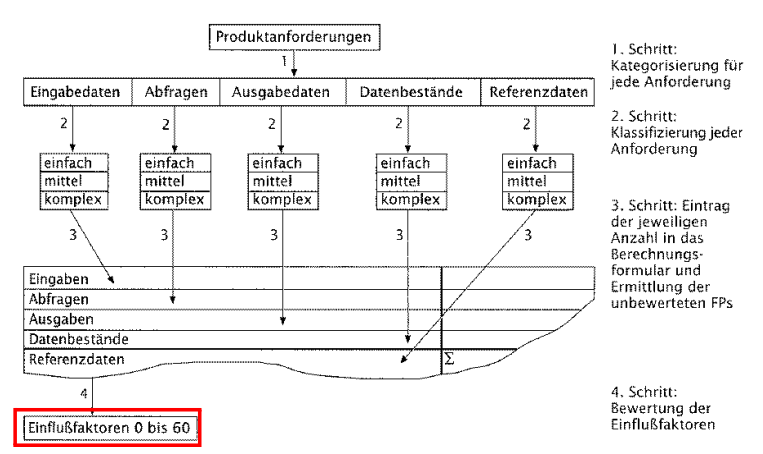
\includegraphics[width=0.85\textwidth]{5_5_1}
\end{figure}

\begin{figure}[h]
\centering
\caption{Überblick über die FP-Methode - 2:}
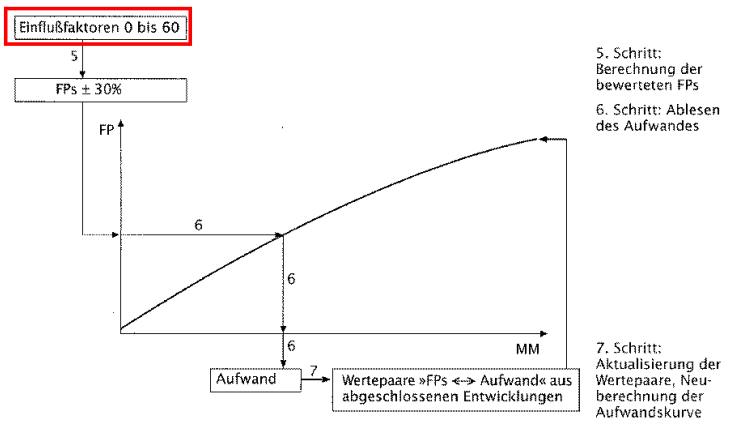
\includegraphics[width=0.85\textwidth]{5_5_2}
\end{figure}

\paragraph{Zusätzliche Einflussfaktoren:}
Die vorige Tabelle unterscheidet sieben Einflussfaktoren; andere Quellen nennen 14 bzw. \textbf{19 verschiedene Faktoren}, die Werte von 0 bis 5 erhalten (siehe [Hu99]):
\begin{enumerate}
	\item Komplexität der Datenkommunikation
	\item Grad der verteilten Datenverarbeitung
	\item geforderte Leistungsfähigkeit
	\item Komplexität der Konfiguration (Zielplattform)
	\item Anforderung an Transaktionsrate
	\item Prozentsatz interaktiver Dateneingaben
	\item geforderte Benutzerfreundlichkeit
	\item interaktive bzw. Online-Pflege des internen Datenbestandes
	\item Komplexität der Verarbeitungslogik
	\item geforderter Grad der Wiederverwendbarkeit
	\item benötigte Installationshilfen
	\item leichte Bedienbarkeit (Grad der Automatisierung der Bedienung)
	\item Mehrfachinstallationen (auf verschiedenen Zielplattformen)
	\item Grad der gefoderten Änderungsfreundlichkeit
	\item Randbedingungen anderer Anwendungen
	\item Sicherheit, Datenschutz, Prüfbarkeit
	\item Anwenderschulung
	\item Datenaustausch mit anderen Anwendungen
	\item Dokumentation
\end{enumerate}

\paragraph{Ermittlung der FP-Aufwandskurve:}
\begin{itemize}
	\item beim ersten Projekt muss man auf \textbf{bekannte Kurven} (für ähnliche Projekte) zurückgreifen (IBM-Kurve mit $FP = 26 * MM^{0,8}8$, VW AG Kurve, ... )
	\item alternativ kann man eigene abgeschlossene Projekte \textbf{nachkalkulieren}, allerdings:
	\begin{itemize}
		\item Nachkalkulationen sind aufwändig
		\item Dokumentation von Altprojekten oft unvollständig
		\item oft gibt es nur noch den Quellcode (keine Lasten- oder Pflichtenhefte)
		\item Kosten (Personenmonate) alter Projekte oft unklar (wurden Überstunden berücksichtigt, welche Aktivitäten wurden mitgezählt, ... )
	\end{itemize}
	\item das Verhältnis von MM zu FP bei abgeschlossenen eigenen Projekten wird zur nachträglichen ''\textbf{Kalibrierung}'' der Kurve benutzt:
	\begin{itemize}
		\item neues Wertepaar wird hinzugefügt oder neues Wertepaar ersetzt ältestes Wertepaar
		\item Frage: was für eine Funktion benutzt man für Interpolation von Zwischenwerten (meist nicht linear, sondern eher quadratisch oder gar exponentiell)
	\end{itemize}
\end{itemize}

\paragraph{Nachkalkulation von Projekten mit ''Backfiring''-Methode:}
Bei alten Projekten gibt es oft nur noch den Quellcode und keine Lasten- oder Pflichtenhefte, aus denen FPs errechnet werden können. In solchen Fällen versucht man FPs aus Quellcode rückzurechnen.
\\
\textbf{Achtung:} LOC in Programmiersprache X pro MM Codierung angeblich nahezu konstant -> damit ist z.B. Produktivität beim Codieren in Smalltalk 4 mal höher als in C

\paragraph{Vorgehensweise bei Kostenschätzung (mit FP-Methode):}
\begin{enumerate}
	\item Festlegung des verwendeten \textbf{Ansatzes}, Bereitstellung von Unterlagen
	\item \textbf{Systemgrenzen} festlegen (was gehört zum Softwaresystem dazu)
	\item \textbf{Umfang} des zu erstellenden Softwaresystems (in FPs) \textbf{messen}
	\item Umrechnung von Umfang (FPs) in \textbf{Aufwand} (MM) mit Aufwandskurve
	\item \textbf{Zuschläge} einplanen (für unvorhergesehene Dinge, Schätzungenauigkeit)
	\item Aufwand auf Phasen bzw. Iterationen \textbf{verteilen}
	\item Umsetzung in \textbf{Projektplan} mit Festlegung von \textbf{Teamgröße}
	\item Aufwandschätzung \textbf{prüfen} und dokumentieren
	\item Aufwandschätzung für Projekt während Laufzeit regelmäßig \textbf{aktualisieren}
	\item Datenbasis für eingesetztes Schätzverfahren aktualisieren, Verfahren \textbf{verbessern}
\end{enumerate}

\paragraph{Einplanung von Zuschlägen (Faustformel nach Augustin):}
Korrekturfaktor $K = 1,8/(1+0,8 F^3)$ für Zuschläge mit F als geschätzter Fertigstellungsgrad der Software.

\paragraph{Problem mit der Berechnung des Fertigstellungsgrades der Software:}
Der Wert F ist vor Projektende unbekannt, muss also selbst geschätzt werden als \textbf{F = bisheriger Aufwand / (bisheriger Aufwand + geschätzter Restaufwand)}

\paragraph{Modifizierte Formel für korrigierte Aufwandsschätzung:}
$MM_{g} = MM_{e} + MM_{k} = MM_{e} + MM_{r}*1,8/(1 + 0,8(MM_{e}/(MM_{e} + MM_{r}))^3)$
\\
\\
$MM_{g}$ = korrigierter geschätzter Gesamtaufwand in Mitarbeitermonaten
\\
$MM_{e}$ = bisher erbrachter Aufwand in Mitarbeitermonaten
\\
$MM_{k}$ = korrigierter geschätzter Restaufwand in Mitarbeitermonaten
\\
$MM_{r}$ = geschätzter Restaufwand in Mitarbeitermonaten
\\

\paragraph{Erläuterungen zu Korrekturfaktor für Kostenschätzung:}
\begin{itemize}
	\item zu \textbf{Projektbeginn} ist F = 0, da noch kein Aufwand erbracht wurde; damit wird der geschätzte Aufwand um 80\% nach oben korrigiert
	\item am \textbf{Projektende} ist F = 1, da spätestens dann die aktuelle Schätzung mit tatsächlichem Wert übereinstimmen sollte, es gibt also keinen Aufschlag mehr
	\item Unsicherheiten in der Schätzung nehmen nicht \textbf{nicht linear} ab, da Wissenszuwachs über zu realisierende Softwarefunktionalität und technische Schwierigkeiten im Projektverlauf keinesfalls linear ist
	\item im Laufe des Projektes wird Fertigstellungsgrad F nicht immer zunehmen, sondern ggf. auch abnehmen, wenn Schätzungen sich als \textbf{zu optimistisch} erwiesen haben
	\item Auftraggeber wird mit Zuschlag von 80\% auf geschätzte Kosten nicht zufrieden sein, deshalb werden inzwischen manchmal Verträge geschlossen, bei denen nur \textbf{Preis je realisiertem FP} vereinbart wird:
	\begin{itemize}
		\item Risiko für zu niedrige Schätzung von FPs liegt bei Auftraggeber
		\item Risiko für zu niedrige Umrechnung v. FPs in MM liegt bei Auftragnehmer
	\end{itemize}
\end{itemize}

\paragraph{Aufwandsverteilung auf Phasen bzw. Entwicklungsaktivitäten:}
Hat man den Gesamtaufwand für ein Softwareentwicklungsprojekt geschätzt, muss man selbst bei einer ersten Grobplanung schon die ungefähre \textbf{Länge einzelner Phasen} oder Iterationen festlegen:
\begin{itemize}
	\item für die Aufteilung des Aufwandes auf Phasen bzw. Aktivitätsbereiche gibt es die \textbf{Prozentsatzmethode}, hier in der Hewlett-Packard-Variante aus [Ba98]:
	\begin{itemize}
		\item Analyseaktivitäten: 18\% des Gesamtaufwandes
		\item Entwurfsaktivitäten: 19\% des Gesamtaufwandes
		\item Codierungsaktivitäten: 34\% des Gesamtaufwandes
		\item Testaktivitäten: 29\% des Gesamtaufwandes
	\end{itemize}
	\item für die Aufwandsberechnung \textbf{einzelner Iterationen} einer Phase wird die Zuordnung von FPs zu diesen Iterationen herangezogen oder es wird bei festgelegter Projektlänge und fester Länge von Iterationen (z.B. 4 Wochen) die Anzahl der FPs, die in einer Iteration zu behandeln sind, festgelegt
\end{itemize}

\paragraph{Bestimmung optimaler Entwicklungsdauer (Faustformel nach Jones):}
für geringen Kommunikationsoverhead und hohen Parallelisierungsgrad: \\
$Dauer = 2,5*(Aufwand in MM)^S$ mit \\
s = 0,38 für Stapel-Systeme \\
s = 0,35 für Online-Systeme \\
s = 0,32 für Echtzeit-Systeme \\
durchschnittliche \textbf{Teamgröße = Aufwand/Dauer}

\textbf{Überlegungen zu obiger Formel:}
\begin{itemize}
	\item Anzahl der maximal sinnvoll parallel arbeitenden Mitarbeiter hängt ab von Projektart
	\item große Projekte dürfen nicht endlos lange laufen (also mehr Mitarbeiter)
	\item mit der Anzahl der Mitarbeiter wächst aber der Kommunikations- und der Verwaltungsaufwand überproportional (also weniger Mitarbeiter)
	\item Anzahl sinnvoll parallel zu beschäftigender Mitarbeiter während Projektlaufzeit (Putnam-Kurve)
\end{itemize}

\paragraph{Bewertung der FP-Methode:}

\begin{itemize}
	\item lange Zeit wurde LOC-basierte Vorgehensweise propagiert
	\item inzwischen: FP-Methode ist wohl einziges halbwegs funktionierendes Schätzverfahren
	\item Abweichungen trotzdem groß (insbesondere bei Einsatz ''fremder'' Kurven)
	\item Anpassung an OO-Vorgehensmodelle, moderne Benutzeroberflächen notwendig
	\item moderne Varianten in Form von ''\textbf{Object-Point-Methode}'', ... sind noch nicht standardisiert und haben sich wohl noch nicht durchgesetzt
	\item Schätzungsfehler in der Machbarkeitsstudie sind nicht immer auf fehlerhafte Schätzmethode zurückzuführen, sondern ggf. auch auf \textbf{nicht} im Lastenheft \textbf{vereinbarte} aber \textbf{realisierte Funktionen} oder zusätzliche Umbaumaßnahmen
	\item bisher geschilderte Vorgehensweise \textbf{nur für Neuentwicklungen} geeignet (ohne umfangreiche Umbaumaßnahmen im Zuge iterativer Vorgehensweise)
\end{itemize}

\paragraph{Problematik der FP-Berechnung bei iterativer Vorgehensweise:}
Bei Projekten zur \textbf{Sanierung oder Erweiterung} von Softwaresystemen bzw. bei einer stark iterativ geprägten Vorgehensweise (mit Umbaumaßnahmen) werden einem System nicht nur Funktionen hinzugefügt, sondern auch Funktionen verändert bzw. entfernt. Damit ergibt sich der Aufwand für Projektdurchführung aus: \\
\textbf{Aufwand in MM = Aufwand für hinzugefügte Funktionen + Aufwand für gelöschte Funktionen + Aufwand für geänderte Funktionen}

\paragraph{Vorgehensweise:}
\begin{itemize}
	\item man benötigt modifizierte Regeln für die Berechnung von FPs für \textbf{gelöschte} Funktionen (Löschen etwas einfacher als Hinzufügen, deshalb weniger FPs?)
\end{itemize}
man benötigt modifizierte Regeln für die Berechnung von FPs für \textbf{geänderte} Funktionen (Ändern = Löschen + Hinzufügen?)
